\subsubsection{Visualizar Agenda}
En la siguiente figura \ref{fig:Diagrama de Secuencia - Visualizar Agenda} se muestra el diagrama de secuencia que corresponde a la visualización de la agenda que el Mecánico (Usuario) tiene en cuanto a los vehículos que va a reparar dentro del taller. Existen dos posibilidades dentro de esta actividad:
\begin{itemize}
	\item \textbf{Si existen registros:} Al momento de que el usuario entra a esta parte del sistema, al existir registros de vehículos por reparar, se muestra toda la información en una tabla y/o lista para su posterior gestión.  
	\item \textbf{No existen registros:} No hay vehículos registrados por reparar, se muestra una tabla y/o lista vacía en pantalla.
\end{itemize}
\begin{figure}[!h]
	\centering
	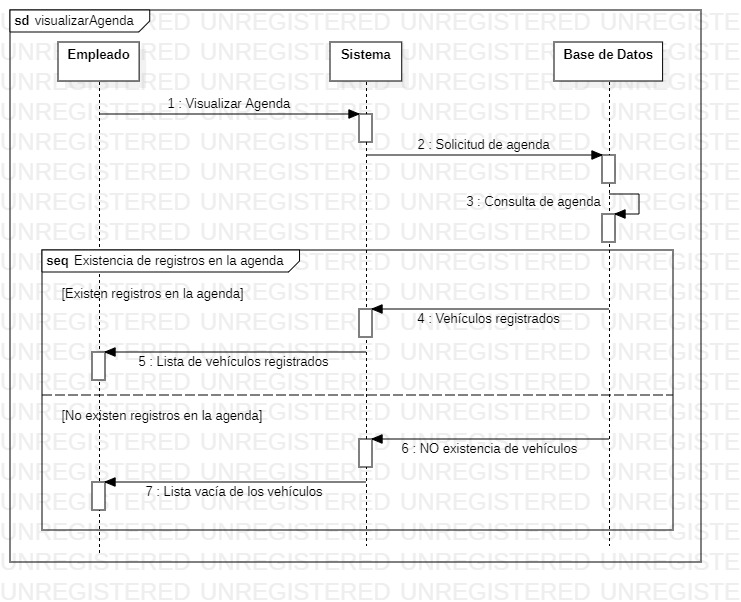
\includegraphics[width=1\textwidth]{./diseno/vprocesos/imagenes/visualizarAgenda}
	\caption{Diagrama de Secuencia - Visualizar Agenda}
	\label{fig:Diagrama de Secuencia - Visualizar Agenda}
\end{figure}